\section{Social and economic impact}

Public scrutiny often targets science funding, demanding evidence of its
tangible social and economic benefits. This challenge is particularly pronounced
in fields like astronomy and astrodynamics, where justifying investments for
exploring distant celestial objects and phenomena is difficult.

A pivotal outcome of the research process lies in the array of technologies
conceived, subsequently finding diverse applications for societal improvement.
Consider the iconic Apollo program as an example. The groundbreaking
technologies developed for the success of Apollo missions, including the
formidable Saturn V rocket, the versatile Lunar Module, and the pioneering
Apollo Guidance Computer (AGC) depicted in Figure \ref{fig:apollo-agc}, have
transcended their original purposes and found invaluable utility across various
fields.

\begin{figure}[H]
  \centering
  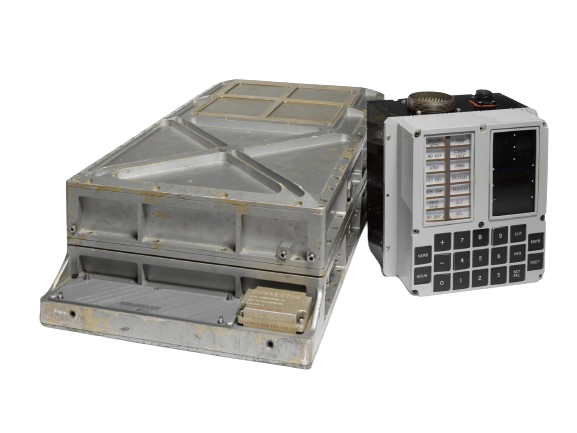
\includegraphics[width=0.7\textwidth]{static/apollo-agc.png}
  \caption[Apollo Guidance Computer]{
  The figure displays two key components of the AGC: the Computer Unit,
  constructed entirely from NOR gate integrated circuits on the left, and
  the Display and Keyboard (DSKY) on the right, used by astronauts to
  interact with the AGC.
  }
  \label{fig:apollo-agc}
\end{figure}

These technologies incorporated novel approaches, notably the utilization of
integrated circuits (ICs). The challenges addressed during this era have paved
the way for modern advancements, evident in the widespread adoption of
fly-by-wire technology in commercial airplanes and the ubiquitous presence of
ICs in various devices.

Similarly, the study of interstellar objects holds promise for fostering
innovation in propulsion, navigation, and observation technologies. These
advancements can be subsequently adapted and applied in other disciplines, such
as Earth observation, satellite communications, and space debris mitigation.
